\documentclass[10pt,a4paper]{article}
\usepackage[T1]{fontenc}\usepackage[utf8]{inputenc}\usepackage{geometry}\geometry{margin=2cm}\usepackage{tikz}
\title{hymeko\_sbsh: the orthtree generic over its coordinate type}\author{HyMeKo graph}
\date{Created-at: 2026-09-24 12:40 CEST}
\begin{document}\maketitle
\textbf{Approval.} This is a core item (\texttt{CORE.YAML}: \texttt{hymeko\_sbsh}). The user directed
it on 2026-09-24: ``Let's make the hymeko\_sbsh generic templates so the types can be set
easily''.

\textbf{Scope.} The design has three parts:
\begin{itemize}
\item a \texttt{Coordinate} trait, implemented for \texttt{f32} and \texttt{f64}, providing
  ordering, \texttt{+}, \texttt{-}, \texttt{*}, \texttt{ZERO}, \texttt{HALF}, \texttt{min} and
  \texttt{max};
\item \texttt{OrthTree<T = f64>}, \texttt{SplitRule<T = f64>}, \texttt{build\_orthtree<T>} and
  \texttt{point\_bbox<T>};
\item \texttt{CountSplit} implements the rule for every \texttt{T}.
\end{itemize}
The arithmetic is unchanged (the midpoint is still $lo\cdot\frac12+hi\cdot\frac12$). The
\texttt{f64} default keeps every caller source-compatible: the scene, \texttt{BoundsIndex} and the
tests. No behaviour change for \texttt{f64}.

\textbf{Tests.}
\begin{itemize}
\item The existing suites pass.
\item New: an \texttt{f32} tree over exactly representable coordinates equals the \texttt{f64}
  tree, in cells, levels, parents, children, members, boxes and \texttt{leaf\_of}, for
  $\dim = 1..3$.
\item New: a generic caller rule.
\end{itemize}

\textbf{Not in scope.} Nagare's own f32 orthtree differs in more than precision: child bit order,
integer-lattice midpoints, the degenerate-split rule, \texttt{leaf\_of} on a dropped orthant, and
the bounding-box padding. Migrating it is a separate decision.

\textbf{Rollback.} Revert the branch.
\begin{center}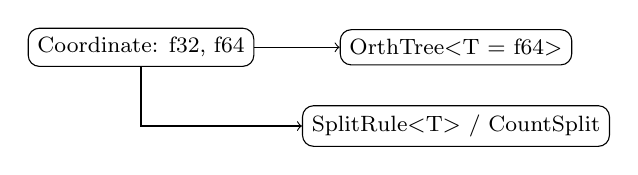
\begin{tikzpicture}[every node/.style={draw,rounded corners,font=\footnotesize}]
\node (c) at (0,0) {Coordinate: f32, f64}; \node (t) at (4,0) {OrthTree$<$T = f64$>$};
\node (r) at (4,-1) {SplitRule$<$T$>$ / CountSplit}; \draw[->] (c)--(t); \draw[->] (c)|-(r);
\end{tikzpicture}
\end{center}
\end{document}
